\subsubsection{Infusion Pump Clamp Design}

The drawings below outline the infusion pump clamp, two are required. Two of these can be fixed together on a stand to provide a clamp for the infusion pump to be fixed to. 
The four bolt and nut holes allow the two parts to be clamped together around the upright support. The internal nut hole and through bolt hole allow a single bolt ant nut to act as grub screw to fix the clamp to the upright support. The two through holes allow bolts to pass through the part to fix the pump to the clamp.


\begin{figure}[h]
    \centering
    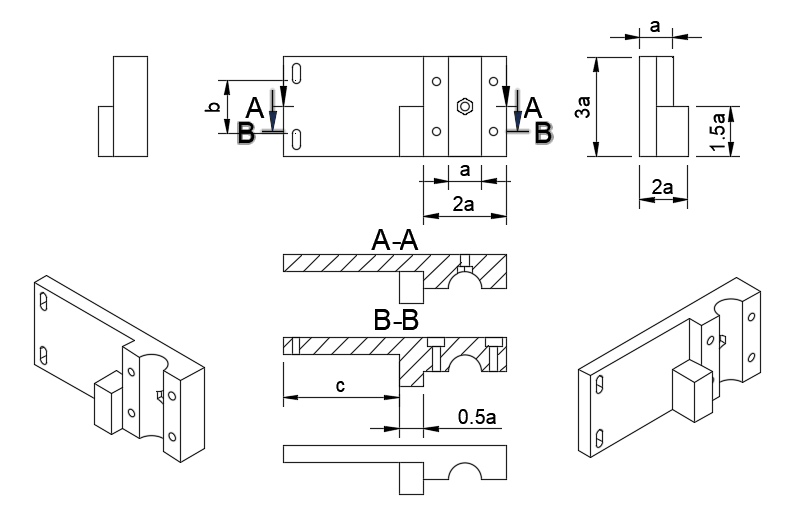
\includegraphics[width=0.7\textwidth]{Figures/SupportDrawings/inf_pump_clamp_drawing.png}
    \caption{Infusion Pump Clamp Drawings}
    \label{fig:infpumpclampdrawing}
  \end{figure}

\begin{enumerate}
  \item[a)]	The diameter of the upright stand/trolley + \textgreater\ 4mm
  \item[b)]	The distance between the pump fixation screw holes - 5mm
  \item[c)]	The length of the pump + \textgreater\ 10mm
\end{enumerate}

